\section{Auswertung}
\label{sec:Auswertung}

\subsection{Vorbereitungsaufgabe} % (fold)
\label{sub:Vorbereitung}

In Vorbereitung auf den Versuch wird herausgesucht bei welchen Energien die Cu-$K_\alpha$- und die Cu-$K_\beta$-Linien
zu erwarten sind und bei welchen Winkeln $\theta$ sie bei Verwendung eines LiF-Kristalls ($d = \qty{201.4}{\pico\meter}$) liegen.
Die Energien liegen bei $E_{K_\alpha,theo}= \qty{8.05}{\kilo\electronvolt}$ und $E_{K_\beta,theo}= \qty{8.91}{\kilo\electronvolt}$\cite{X-Ray}.
Durch Umstellen von \autoref{eqn:Bragg} zu
\begin{align}
  \theta = \arcsin{\frac{h \cdot c} {E \cdot 2 d}} \label{eqn:theta}
\end{align}
wird der Glanzwinkel berechnet zu $\theta_{K_\alpha}= \qty{22.48}{\degree}$ und $\theta_{K_\beta}= \qty{20.21}{\degree}$.

Zudem wird die Ordnungszahl und Energie der K-Kante für die zu untersuchenden Materialien harausgesucht. Mithilfe von
\autoref{eqn:theta} wird der Glanzwinkel bestimmt und mithilfe von \autoref{eqn:sigmak} die Abschirmkonstante berechnet.
Die Ergebnisse sind in \autoref{tab:Vorbereitung} aufgetragen.

\begin{table}[H]
  \centering
  \caption{Literaturwerte und daraus berechnete Größen verschiedener Elemente.\cite{X-Ray}}
  \label{tab:Vorbereitung}
  \sisetup{table-format=2.2}
  \begin{tabular}{c S[table-format=2.0] S S S[table-format=1.2] }
  \toprule
  {Element} & {Z} & {$E_{K}^{lit} [\si{\kilo\electronvolt}]$}& {$\theta_{K}^{lit} [\si{\degree}]$} & {$\sigma_K$}\\
  \midrule
    Zn & 30 &  9.65 & 18.60 & 3.56 \\
    Ge & 32 & 11.11 & 16.08 & 3.66 \\
    Br & 35 & 13.48 & 13.20 & 3.84 \\
    Rb & 37 & 15.21 & 11.68 & 3.93 \\
    Sr & 38 & 16.12 & 11.01 & 3.98 \\
    Zr & 40 & 18.01 &  9.84 & 4.08 \\
    Ga & 31 & 10.38 & 17.25 & 3.60 \\ 
  \bottomrule
  \end{tabular}
\end{table}
% subsection  (end)

\subsection{Überprüfung der Bragg-Bedingung} % (fold)
\label{sub:Bragg_aus}
Die Messung wird nach \autoref{sub:Bragg_durch} durchgeführt.
Aus den gemessenen Daten wird das Maximum der Kurve bestimmt und mit dem Sollwinkel verglichen.
\begin{figure}[H]
  \centering
  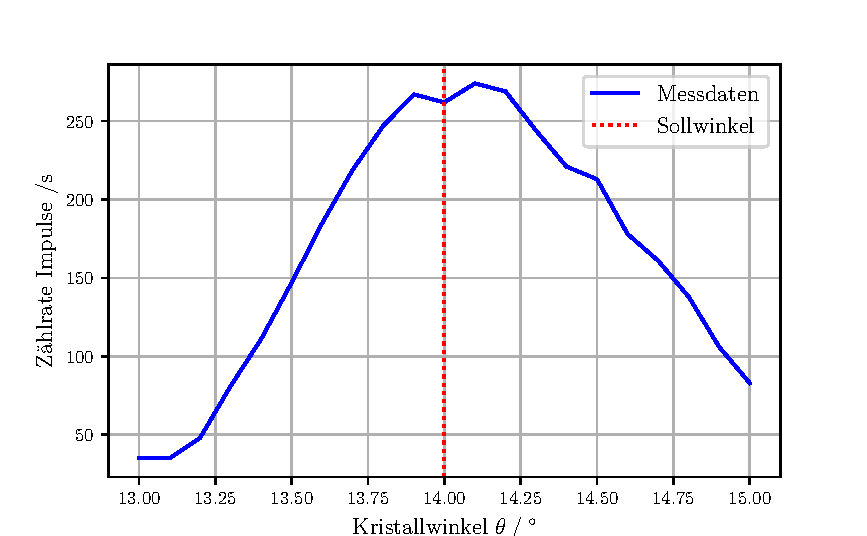
\includegraphics[width=\textwidth]{build/plot1.pdf}
  \caption{Emissionsspektrum bei festem Kristallwinkel von $\theta = \qty{14}{\degree}$.}
  \label{fig:plot1}
\end{figure}

Das Maximum der Kurve in \autoref{fig:plot1} liegt bei $\theta=\qty{14.1}{\degree}$.

% subsection Überprüfung der Bragg-Bedingung (end)

\subsection{Analyse des Emissionsspektrums einer Cu-Röntgenröhre} % (fold)
\label{sub:Emission_aus}

\begin{figure}[H]
  \centering
  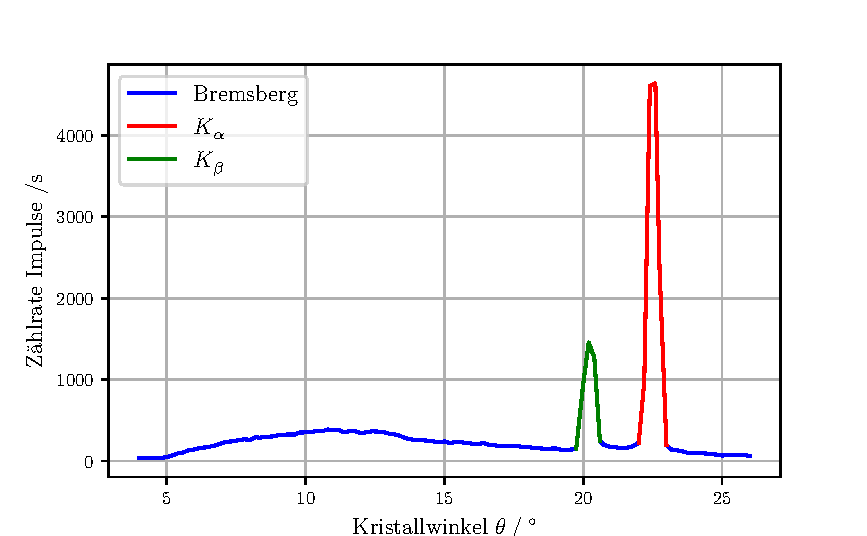
\includegraphics[width=\textwidth]{build/plot2.pdf}
  \caption{Emissionsspektrum der Cu-Röntgenröhre.}
  \label{fig:plot2}
\end{figure}

Die Maxima der Kurve und somit die Winkel für die Energien liegen für die 
$K_\alpha$ -Energie  bei $\theta_\alpha=\qty{22.6}{\degree}$ und für die $K_\beta$ - Energie
bei $\theta_\beta=\qty{20.2}{\degree}$.
Daraus folgen nach \autoref{eqn:Bragg} die Energien
\begin{align*}
  E_{K_\alpha}&= \qty{8.01}{\kilo\electronvolt}\\
  E_{K_\beta}&= \qty{8.91}{\kilo\electronvolt}
\end{align*} 


Aus \autoref{fig:plot2} werden außerdem die Halbwertsbreiten der $K_\alpha$ - Linie zu $\Delta\theta_{\alpha,halb}=\qty{0.6}{\degree}$ und
der $K_\beta$ - Linie zu $\Delta\theta_{\beta,halb}=\qty{0.4}{\degree}$ bestimmt.
Mit den entsprechenden Werten  
\begin{align*}
  \theta_{\alpha,halb1}&=\qty{22.3}{\degree}  & E_{\alpha,halb1}&= \qty{8.11}{\kilo\electronvolt}\\
  \theta_{\alpha,halb2}&=\qty{22.7}{\degree}  & E_{\alpha,halb2}&= \qty{7.98}{\kilo\electronvolt}\\
  \theta_{\beta,halb1}&=\qty{19.9}{\degree}    & E_{\beta,halb1}&= \qty{9.04}{\kilo\electronvolt}\\
  \theta_{\beta,halb2}&=\qty{20.5}{\degree}  & E_{\beta,halb2}&= \qty{8.79}{\kilo\electronvolt}
 \end{align*}
wird die Energiedifferenz
\begin{align*}
 \Delta E_{\alpha,halb}&= \qty{0.13}{\kilo\electronvolt}\\
 \Delta E_{\beta,halb}&= \qty{0.25}{\kilo\electronvolt}
\end{align*}
berechnet.
Das Auflösungsvermögen beträgt nach 
\begin{align*}
  A &= \frac{E_K}{\Delta E}:
\end{align*}
\begin{align*}
  A_{K_\alpha} &= 61.62\\
  A_{K_\beta} &= 35.64.
\end{align*}


Die Abschirmkonstanten werden mit \autoref{eqn:Ekabs} bis \autoref{eqn:Ekb} bestimmt. Hierbei wird
$E_{K,abs}= \qty{8.99}{\kilo\electronvolt}$\cite{X-Ray} verwendet, was durch den Versuchsaufbau nicht bestimmt werden kann.
Außerdem gilt $n=1, m=2$ und $l=3$.
Somit berechnen sich die Abschirmkontanten zu
\begin{align*}
  \sigma_1 &= 3.29\\
  \sigma_2 &= 12.02\\
  \sigma_3 &= 21.72.
\end{align*}
% subsection Das Emissionsspektrum einer Cu-Röntgenröhre (end)

\subsection{Analyse der Absorptionsspektren} % (fold)
\label{sub:Absorption_aus}
Die Messung wird wie in \autoref{sub:Absorption_durch} beschrieben durchgeführt.
In \autoref{fig:plot3} bis \ref{fig:plot7} sind die Absorptionsspektren der fünf Materialien dargestellt.
Aus denen knenn die Winkel abgelesen werden, bei denen die K-Kanten auftreten.
Diese werden in \autoref{tab:Absorption_aus} eingetragen und mit diesen Winkeln wird die Absorptionsenergie mit \autoref{eqn:Ekabs} berechnet.
Außerdem wird mit diesen Winkeln und den Absorptionsenergien die Abschirmzahlen $\sigma_K$ mit \autoref{eqn:sigmak} bestimmt.
Die bestimmten Zahlen werden der \autoref{tab:Absorption_aus} hinzugefügt.

\begin{table}[H]
  \centering
  \caption{Gemessen Kristallwinkel und daraus bestimmten Werte.}
  \label{tab:Vorbereitung}
  \sisetup{table-format=2.2}
  \begin{tabular}{c S[table-format=2.0] S S S[table-format=1.2] }
  \toprule
  {Element} & {Abbildung} & {$\theta_{K}^{lit} [\si{\degree}]$} & {$E_{K}^{lit} [\si{\kilo\electronvolt}]$}& {$\sigma_K$}\\
  \midrule
    Zn & 7 &  9.65 & 18.60 & 3.56 \\
    Sr & 8 & 16.12 & 11.01 & 3.98 \\
    Zr & 9 & 18.01 &  9.84 & 4.08 \\
    Br & 10 & 13.48 & 13.20 & 3.84 \\
    Ga & 11 & 10.38 & 17.25 & 3.60 \\ 
  \bottomrule
  \end{tabular}
\end{table}

\begin{figure}[H]
  \centering
  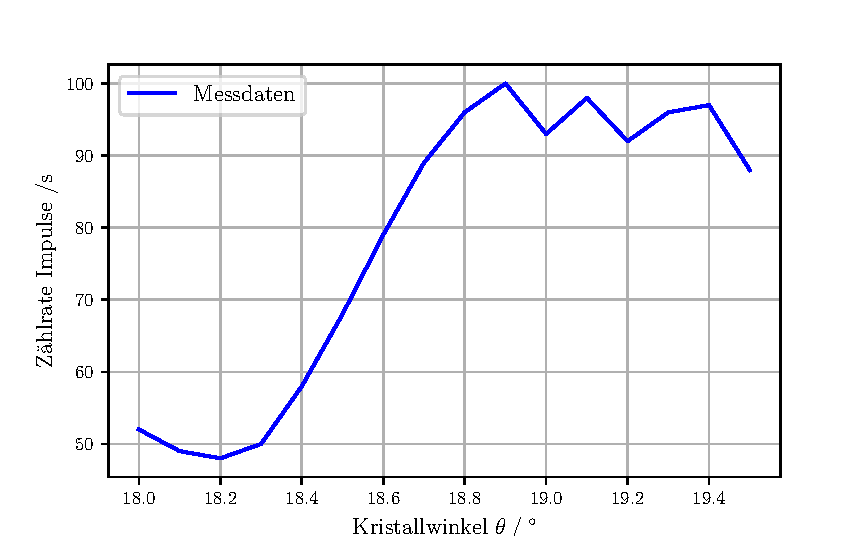
\includegraphics[width=\textwidth]{build/plot3.pdf}
  \caption{Absorptionsspektrum von Zink.}
  \label{fig:plot3}
\end{figure}

\begin{figure}[H]
  \centering
  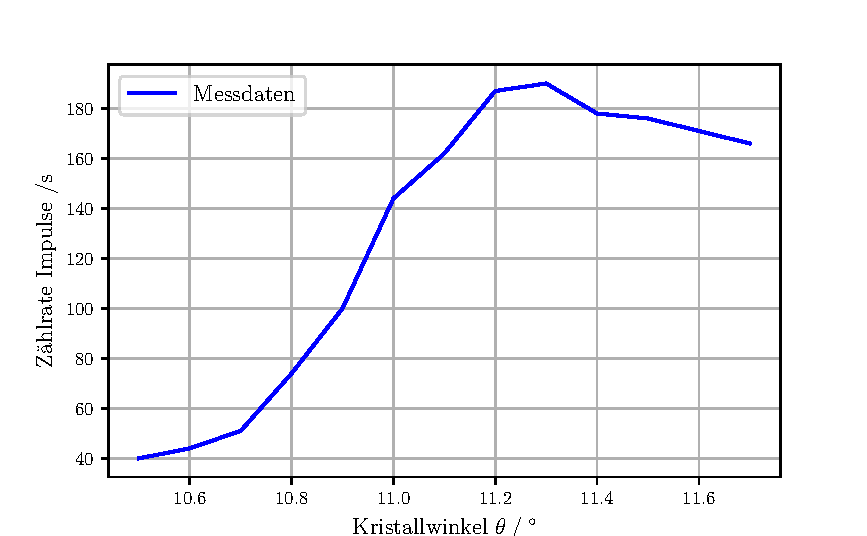
\includegraphics[width=\textwidth]{build/plot4.pdf}
  \caption{Absorptionsspektrum von Strontium.}
  \label{fig:plot4}
\end{figure}

\begin{figure}[H]
  \centering
  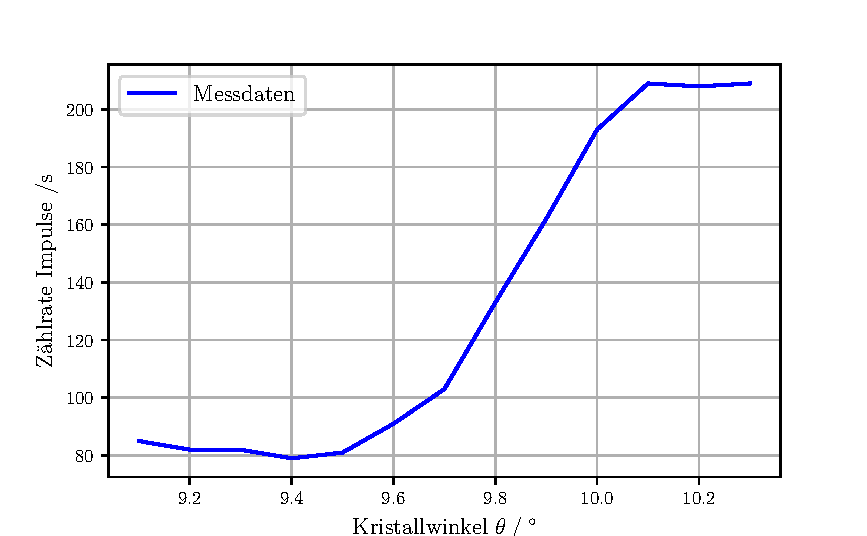
\includegraphics[width=\textwidth]{build/plot5.pdf}
  \caption{Absorptionsspektrum von Zirkonium.}
  \label{fig:plot5}
\end{figure}

\begin{figure}[H]
  \centering
  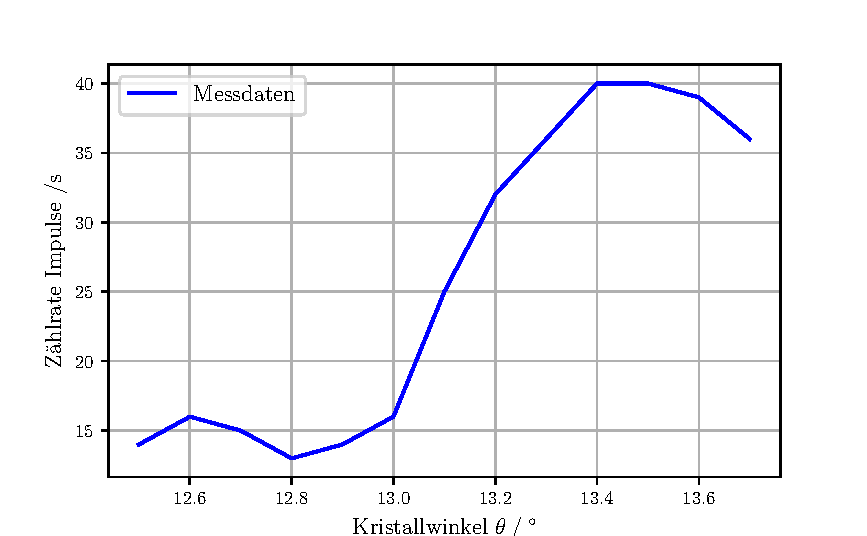
\includegraphics[width=\textwidth]{build/plot6.pdf}
  \caption{Absorptionsspektrum von Brom.}
  \label{fig:plot6}
\end{figure}

\begin{figure}[H]
  \centering
  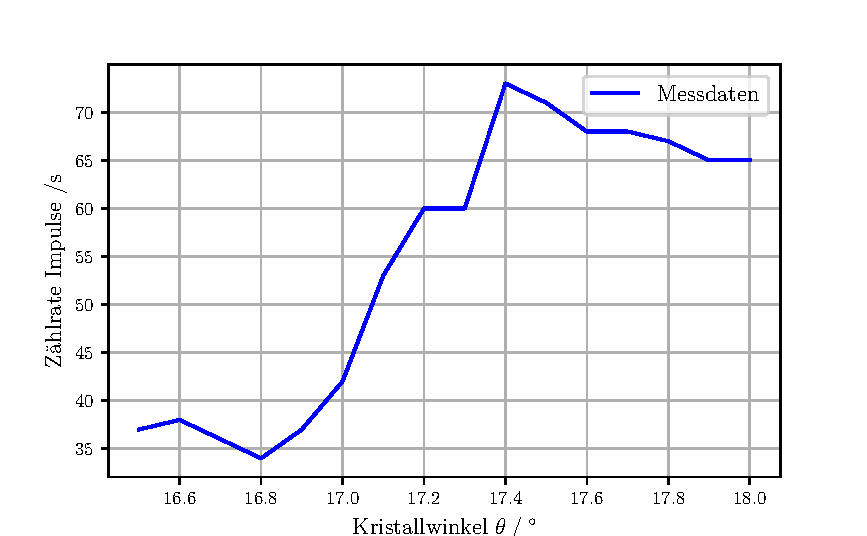
\includegraphics[width=\textwidth]{build/plot7.pdf}
  \caption{Absorptionsspektrum von Gallium.}
  \label{fig:plot7}
\end{figure}

Zink Maximum bei 18.9 Minimum 18.2
Strontium Maximum 11.3 Minimum 10.5
Zirkonium Maximum 10.1 Minimum 9.4
Brom Maximum 13.4 Minimum 12.8
Gallium Maximum 17.4 Minimum 16.8
% subsection Das Absorptionsspektrum (end)